\newcommand{\svcourse}{CST Part IA: Software Engineering and Security}
\newcommand{\svnumber}{1}
\newcommand{\svvenue}{Microsoft Teams}
\newcommand{\svdate}{2022-05-11}
\newcommand{\svtime}{15:00}
\newcommand{\svuploadkey}{CBd13xmL7PC1zqhNIoLdTiYUBnxZhzRAtJxv/ytRdM1r7qIfwMsxeVwM/pPcIo8l}

\newcommand{\svrname}{Dr Sam Ainsworth}
\newcommand{\jkfside}{oneside}
\newcommand{\jkfhanded}{yes}

\newcommand{\studentname}{Harry Langford}
\newcommand{\studentemail}{hjel2@cam.ac.uk}


\documentclass[10pt,\jkfside,a4paper]{article}

\usepackage{tikz}
\usepackage{graphicx}
\usepackage{float}
\usetikzlibrary{arrows.meta, calc, positioning}

% DO NOT add \usepackage commands here.  Place any custom commands
% into your SV work files.  Anything in the template directory is
% likely to be overwritten!

\usepackage{fancyhdr}

\usepackage{lastpage}       % ``n of m'' page numbering
\usepackage{lscape}         % Makes landscape easier

\usepackage{verbatim}       % Verbatim blocks
\usepackage{listings}       % Source code listings
\usepackage{graphicx}
\usepackage{float}
\usepackage{epsfig}         % Embed encapsulated postscript
\usepackage{array}          % Array environment
\usepackage{qrcode}         % QR codes
\usepackage{enumitem}       % Required by Tom Johnson's exam question header

\usepackage{hhline}         % Horizontal lines in tables
\usepackage{siunitx}        % Correct spacing of units
\usepackage{amsmath}        % American Mathematical Society
\usepackage{amssymb}        % Maths symbols
\usepackage{amsthm}         % Theorems

\usepackage{ifthen}         % Conditional processing in tex

\usepackage[top=3cm,
            bottom=3cm,
            inner=2cm,
            outer=5cm]{geometry}

% PDF metadata + URL formatting
\usepackage[
            pdfauthor={\studentname},
            pdftitle={\svcourse, SV \svnumber},
            pdfsubject={},
            pdfkeywords={9d2547b00aba40b58fa0378774f72ee6},
            pdfproducer={},
            pdfcreator={},
            hidelinks]{hyperref}

\renewcommand{\headrulewidth}{0.4pt}
\renewcommand{\footrulewidth}{0.4pt}
\fancyheadoffset[LO,LE,RO,RE]{0pt}
\fancyfootoffset[LO,LE,RO,RE]{0pt}
\pagestyle{fancy}
\fancyhead{}
\fancyhead[LO,RE]{{\bfseries \studentname}\\\studentemail}
\fancyhead[RO,LE]{{\bfseries \svcourse, SV~\svnumber}\\\svdate\ \svtime, \svvenue}
\fancyfoot{}
\fancyfoot[LO,RE]{For: \svrname}
\fancyfoot[RO,LE]{\today\hspace{1cm}\thepage\ / \pageref{LastPage}}
\fancyfoot[C]{\qrcode[height=0.8cm]{\svuploadkey}}
\setlength{\headheight}{22.55pt}


\ifthenelse{\equal{\jkfside}{oneside}}{

 \ifthenelse{\equal{\jkfhanded}{left}}{
  % 1. Left-handed marker, one-sided printing or e-marking, use oneside and...
  \evensidemargin=\oddsidemargin
  \oddsidemargin=73pt
  \setlength{\marginparwidth}{111pt}
  \setlength{\marginparsep}{-\marginparsep}
  \addtolength{\marginparsep}{-\textwidth}
  \addtolength{\marginparsep}{-\marginparwidth}
 }{
  % 2. Right-handed marker, one-sided printing or e-marking, use oneside.
  \setlength{\marginparwidth}{111pt}
 }

}{
 % 3. Alternating margins, two-sided printing, use twoside.
}


\setlength{\parindent}{0em}
\addtolength{\parskip}{1ex}

% Exam question headings, labels and sensible layout (courtesy of Tom Johnson)
\setlist{parsep=\parskip, listparindent=\parindent}
\newcommand{\examhead}[3]{\section{#1 Paper #2 Question #3}}
\newenvironment{examquestion}[3]{
\examhead{#1}{#2}{#3}\setlist[enumerate, 1]{label=(\alph*)}\setlist[enumerate, 2]{label=(\roman*)}
\marginpar{\href{https://www.cl.cam.ac.uk/teaching/exams/pastpapers/y#1p#2q#3.pdf}{\qrcode{https://www.cl.cam.ac.uk/teaching/exams/pastpapers/y#1p#2q#3.pdf}}}
\marginpar{\footnotesize \href{https://www.cl.cam.ac.uk/teaching/exams/pastpapers/y#1p#2q#3.pdf}{https://www.cl.cam.ac.uk/\\teaching/exams/pastpapers/\\y#1p#2q#3.pdf}}
}{}


\begin{document}

\begin{examquestion}{2001}{9}{1}

\begin{enumerate}[label=(\alph*)]

\item Explain the problem of clock drift in distributed systems.

The clock in nodes in distributed systems are not perfect. Some run
slightly faster and some slightly slower. The rate by which a clock runs
fast or slow is its drift. After a long time, clocks can become out-of-sync
and be no longer be monotonic -- we can send a message and from the
perspective of the recipient, it can have been from the future.

\item What sources of conventional earth time might be used by computer
systems? How would you estimate bounds on the accuracy of time received from
such a source?

Conventional earth time can be determined from GPS\@. Geostationary
satellites have caesium-133 atomic clocks. These geostationary satellites
orbit the planet and broadcast the current time and their position. A
server can then hear the signal from multiple satellites and using the
delay between them, work out its own position and the current time. You can
estimate bounds on the accuracy by repeating the process multiple times or
repeating with different satellites.

\item What constraint does distributed inter-process communication (IPC)
impose on the clock values of the communicating parties?

Distributed inter-process communication requires that each parties clock
respects causality.

\item Outline one clock synchronisation protocol that satisfies this
constraint.

Vector clocks respect causality. A vector clock keeps track of the last
operation each node did that could have affected the current process. Vector
clocks do not use physical time, but logical time.

A vector clock timestamp in a system with $n$ nodes is a $n$-dimensional
vector where the $n^{\text{th}}$ dimension represents the last known
operation at node $n$.

If Node $i$ has vector timestamp $t$ then here are the protocols for
operations:

\begin{itemize}

\item To send a message, increment $t[i]$ then send the message along with
the new timestamp

\item On receiving a message with timestamp $t'$, take the elementwise
maximum of $t'$ and $t$. Let this be $t''$. Increment $t''[i]$ and let $t''$
be the new timestamp.

\end{itemize}

If we have two timestamps, $T_1$ and $T_2$ then $T_1 < T_2$ if and only if
$(\forall i. T_1[i] \leq T_2[i]) \wedge (\exists i. T_1[i] < T_2[i])$.

If we have two timestamps $T_1$ and $T_2$ such that $T_1 \not< T_2 \wedge
T_2 \not< T_1$ then we say that $T_1$ and $T_2$ are concurrent, denoted
$T_1 \| T_2$.

\item For each of the cases of IPC illustrated below, give the vector clock
values that message receiving modules and delivery modules could maintain
for each process.

\begin{enumerate}

\item
\begin{center}
\begin{tikzpicture}
\node (P0) {$P_0$};
\node (P1) [below = of P0] {$P_1$};
\node (P2) [below = of P1] {$P_2$};
\path (P0) edge ($(P0) + (7,0)$);
\path (P1) edge ($(P1) + (7,0)$);
\path (P2) edge ($(P2) + (7,0)$);
\path [Circle-stealth, shorten <=-2pt] ($(P0) + (1, 0)$) edge ($(P1) + (2,0)$);
\path [Circle-stealth, shorten <=-2pt] ($(P1) + (3, 0)$) edge ($(P2) + (4,0)$);
\path [Circle-stealth, shorten <=-2pt] ($(P0) + (5, 0)$) edge ($(P2) + (6,0)$);
\node (p0leave1) [right = 1 of P0, above]
{$\begin{pmatrix} 1 \\ 0 \\ 0 \\ \end{pmatrix}$};
\node (p1arrive) [right = 2 of P1, above]
{$\begin{pmatrix} 1 \\ 1 \\ 0 \\ \end{pmatrix}$};
\node (p1leave) [right = 3 of P1, above]
{$ \begin{pmatrix} 1 \\ 2 \\ 0 \\ \end{pmatrix} $};
\node (p2arrive1) [right = 4 of P2, above]
{$ \begin{pmatrix} 1 \\ 2 \\ 1 \\ \end{pmatrix} $};
\node (p0leave1) [right = 5 of P0, above]
{$\begin{pmatrix} 2 \\ 0 \\ 0 \\ \end{pmatrix}$};
\node (p2arrive2) [right = 6 of P2, above]
{$ \begin{pmatrix} 2 \\ 2 \\ 2 \\ \end{pmatrix} $};
\end{tikzpicture}
\end{center}

\vspace{1cm}

\item
\begin{center}
\begin{tikzpicture}
\node (P0) {$P_0$};
\node (P1) [below = of P0] {$P_1$};
\node (P2) [below = of P1] {$P_2$};
\path (P0) edge ($(P0) + (7,0)$);
\path (P1) edge ($(P1) + (7,0)$);
\path (P2) edge ($(P2) + (7,0)$);
\path [Circle-stealth, shorten <=-2pt] ($(P0) + (1, 0)$) edge ($(P2) + (6,0)$);
\path [Circle-stealth, shorten <=-2pt] ($(P0) + (2, 0)$) edge ($(P1) + (3,0)$);
\path [Circle-stealth, shorten <=-2pt] ($(P1) + (4, 0)$) edge ($(P2) + (5,0)$);
\node (p0leave1) [right = 1 of P0, above]
{$\begin{pmatrix} 1 \\ 0 \\ 0 \\ \end{pmatrix}$};
\node (p0leave2) [right = 2 of P0, above]
{$\begin{pmatrix} 2 \\ 0 \\ 0 \\ \end{pmatrix}$};
\node (p1arrive) [right = 3 of P1, above]
{$\begin{pmatrix} 2 \\ 1 \\ 0 \\ \end{pmatrix}$};
\node (p1leave) [right = 4 of P1, above]
{$\begin{pmatrix} 2 \\ 2 \\ 0 \\ \end{pmatrix}$};
\node (p2arrive1) [right = 5 of P2, above]
{$\begin{pmatrix} 2 \\ 2 \\ 1 \\ \end{pmatrix}$};
\node (p2arrive1) [right = 6 of P2, above]
{$\begin{pmatrix} 2 \\ 2 \\ 2 \\ \end{pmatrix}$};
\end{tikzpicture}
\end{center}

\vspace{1cm}

\item
\begin{center}
\begin{tikzpicture}
\node (P0) {$P_0$};
\node (P1) [below = of P0] {$P_1$};
\node (P2) [below = of P1] {$P_2$};
\path (P0) edge ($(P0) + (7,0)$);
\path (P1) edge ($(P1) + (7,0)$);
\path (P2) edge ($(P2) + (7,0)$);
\path [Circle-stealth, shorten <=-2pt] ($(P0) + (1, 0)$) edge ($(P2) + (2,0)$);
\path [Circle-stealth, shorten <=-2pt] ($(P0) + (1, 0)$) edge ($(P1) + (3,0)$);
\path [Circle-stealth, shorten <=-2pt] ($(P1) + (4, 0)$) edge ($(P0) + (5,0)$);
\path [Circle-stealth, shorten <=-2pt] ($(P1) + (4, 0)$) edge ($(P2) + (5,0)$);
\node (p0leave) [right = 1 of P0, above]
{$\begin{pmatrix} 1 \\ 0 \\ 0 \\ \end{pmatrix}$};
\node (p1arrive) [right = 3 of P1, above]
{$\begin{pmatrix} 1 \\ 1 \\ 0 \\ \end{pmatrix}$};
\node (p2arrive1) [right = 2 of P2, above]
{$\begin{pmatrix} 1 \\ 0 \\ 1 \\ \end{pmatrix}$};
\node (p1leave) [right = 4 of P1, above]
{$\begin{pmatrix} 1 \\ 2 \\ 0 \\ \end{pmatrix}$};
\node (p0arrive) [right = 5 of P0, above]
{$\begin{pmatrix} 2 \\ 2 \\ 0 \\ \end{pmatrix}$};
\node (p2arrive) [right = 5 of P2, above]
{$\begin{pmatrix} 1 \\ 2 \\ 2 \\ \end{pmatrix}$};
\end{tikzpicture}
\end{center}

\vspace{1cm}

\item
\begin{center}
\begin{tikzpicture}
\node (P0) {$P_0$};
\node (P1) [below = of P0] {$P_1$};
\node (P2) [below = of P1] {$P_2$};
\path (P0) edge ($(P0) + (7,0)$);
\path (P1) edge ($(P1) + (7,0)$);
\path (P2) edge ($(P2) + (7,0)$);
\path [Circle-stealth, shorten <=-2pt] ($(P0) + (1, 0)$) edge ($(P1) + (2,0)$);
\path [Circle-stealth, shorten <=-2pt] ($(P0) + (1, 0)$) edge ($(P2) + (6,0)$);
\path [Circle-stealth, shorten <=-2pt] ($(P1) + (3, 0)$) edge ($(P0) + (5,0)$);
\path [Circle-stealth, shorten <=-2pt] ($(P1) + (3, 0)$) edge ($(P2) + (4,0)$);
\node (p0leave) [right = 1 of P0, above]
{$\begin{pmatrix} 1 \\ 0 \\ 0 \\ \end{pmatrix}$};
\node (p1arrive) [right = 2 of P1, above]
{$\begin{pmatrix} 1 \\ 1 \\ 0 \\ \end{pmatrix}$};
\node (p1leave) [right = 3 of P1, above]
{$\begin{pmatrix} 1 \\ 2 \\ 0 \\ \end{pmatrix}$};
\node (p0arrive) [right = 5 of P0, above]
{$\begin{pmatrix} 2 \\ 2 \\ 0 \\ \end{pmatrix}$};
\node (p2arrive1) [right = 4 of P2, above]
{$\begin{pmatrix} 1 \\ 2 \\ 1 \\ \end{pmatrix}$};
\node (p2arrive2) [right = 6 of P2, above]
{$\begin{pmatrix} 1 \\ 2 \\ 2 \\ \end{pmatrix}$};
\end{tikzpicture}
\end{center}

\end{enumerate}

\item Define ``causal order'' of message delivery. In which, if any, of
($i$) to ($iv$) above is causal order violated at the message receiving module?

Causal order of message delivery means that the order of message delivery
cannot violate the ``happens-before'' relation of the times the messages
were sent.

Informally this means that a message $a$ sent to node $n$ cannot be delivered
until all messages sent to node $n$ which were logically sent before $a$ have
been delivered.

Using vector clocks, causal order of message delivery is violated if a
message with timestamp $t'$ is delivered to a node with timestamp $t$ such
that $\forall i. t'[i] < t[i]$.

Only $ii$ violates causal order of message delivery.

In $ii$, the message sent from $P_0$ to $P_2$ logically happens before the
message sent from $P_0$ to $P_1$. Therefore by transitivity of the
happens-before relation, it logically happens before the message from $P_1$
to $P_2$. However, the message from $P_0$ to $P_2$ was delivered after the
message from $P_1$ to $P_2$. Therefore it was delivered out-of-order.

Note that $iv$ does not violate causal order of message delivery since the
first and second message happened concurrently.

\end{enumerate}

\end{examquestion}

\begin{examquestion}{2005}{9}{4}

\begin{figure}[H]
\centering
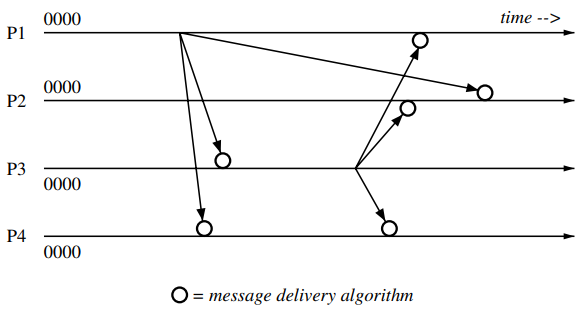
\includegraphics[width=0.8\textwidth]{./examquestion2005_9_4_multicast_diagram}
\end{figure}

The above diagram represents a process group that communicates by means of
multicast messages. At each process-hosting node, message delivery software
decides whether a given incoming message should be delivered to the process
or buffered for later delivery. This is achieved by the use of vector clocks.

\begin{enumerate}[label=(\alph*)]

\item Describe, by means of the above example, the vector clock algorithm
for delivery of messages in causal order.

The vector clock algorithm can be used to ensure broadcast messages are
delivered in causal order.

Each node $i$ has a vector $\mathbf{v}_i$ of size $n$ where $n$ is the number
of processes in the system. The vector clock algorithm maintains the
invariant that $\mathbf{v}_i[j]$ is the number of messages sent from node
$j$ which node $i$ has received.

When node $i$ wishes to broadcast a message, it includes its node id ($i$)
and a copy of $\mathbf{v}_i$ in the message and \textit{then} increments
$\mathbf{v}_i[i]$. The vector timestamp shall be used as a list of
``dependencies'' before the message can be delivered.

When node $i$ receives a message, it adds it to a set of waiting messages.
Then node $i$ checks for any messages with a dependency list that is
satisfied by its current timestamp. If it finds any, it delivers them and
increments $\mathbf{v}_i[j]$ to maintain the invariant that
$\mathbf{v}_i[j]$ is the number of messages delivered to process $i$ which
were sent by process $j$.

\begin{figure}[H]
\centering
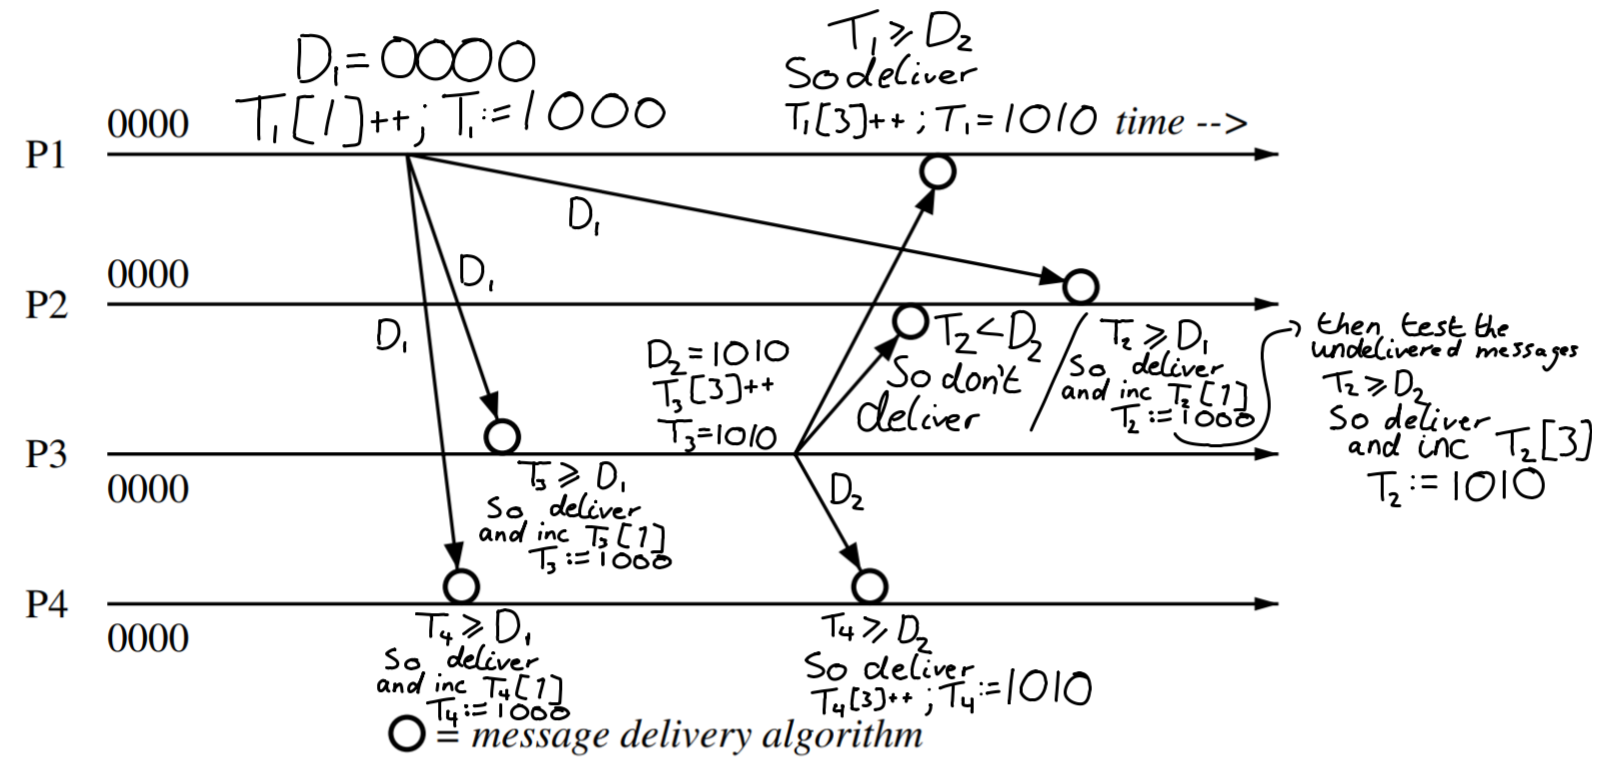
\includegraphics[width=0.8\textwidth]{./vector_clock_causal_order_delivery}
\end{figure}

\item By means of a similar example, show that total ordering of messages is
not achieved by this algorithm.

Consider the below example.

\begin{center}
\begin{tikzpicture}
\node (P0) {$P_0$};
\node (P1) [below = of P0] {$P_1$};
\node (P2) [below = of P1] {$P_2$};
\node (P3) [below = of P2] {$P_3$};
\path (P0) edge ($(P0) + (7,0)$);
\path (P1) edge ($(P1) + (7,0)$);
\path (P2) edge ($(P2) + (7,0)$);
\path (P3) edge ($(P3) + (7,0)$);
\path [Circle-stealth, shorten <=-2pt] ($(P0) + (1, 0)$) edge ($(P1) + (6,0)$);
\path [Circle-stealth, shorten <=-2pt] ($(P0) + (1, 0)$) edge ($(P2) + (2,0)$);
\path [Circle-stealth, shorten <=-2pt, dashed] ($(P0) + (1, 0)$) edge ($(P3)
+ (1.5,0)$);
\path [Circle-stealth, shorten <=-2pt] ($(P3) + (1, 0)$) edge ($(P1) + (4,0)$);
\path [Circle-stealth, shorten <=-2pt] ($(P3) + (1, 0)$) edge ($(P2) + (6,0)$);
\path [Circle-stealth, shorten <=-2pt, dashed] ($(P3) + (1, 0)$) edge ($(P0)
+ (1.5,0)$);
\node (p1arrive1) [right = 6 of P1, above]
{$\begin{pmatrix} 0 \\ 0 \\ 0 \\ 1 \\ \end{pmatrix}$};
\node (p0leave1) [right = 1.5 of P2]
{$\begin{pmatrix} 1 \\ 0 \\ 0 \\ 0 \\ \end{pmatrix}$};
\node (p1arrive1) [right = 4 of P1, above]
{$\begin{pmatrix} 1 \\ 0 \\ 0 \\ 1 \\ \end{pmatrix}$};
\node (p0leave1) [right = 5.5 of P2]
{$\begin{pmatrix} 1 \\ 0 \\ 0 \\ 1 \\ \end{pmatrix}$};
\end{tikzpicture}
\end{center}

In this example, $P_0$ and $P_3$ send messages concurrently and therefore
any order of delivery will respect causal order. In this case, processes
$P_1$ and $P_2$ deliver in two different orders which both respect causal
order. This demonstrates that the vector clock algorithm does not enforce
a total order. Note that to avoid clutter, I have only written the
most important timestamps.

\end{enumerate}

\end{examquestion}

\begin{examquestion}{2004}{8}{4}

\begin{enumerate}[label=(\alph*)]

\item Define strong and weak consistency.

Strong consistency (linearizability) means that every operation takes place
atomically at some point after it started and before it finished.

Weak consistency (serialisability) means that operations have the same
effect as if they were executed in some serial order.

Informally, weak consistency respects only the happens-before relation,
while strong consistency also respects real-time.

\iffalse

Strong consistency (linearizability) means that every operation takes place
atomically at some time after the operation started and before it finished.

Weak consistency (serialisability) means that the operations have the same
effect as though they had been executed in some serial order.

\fi

\item A process group manages a set of widely distributed replicas. The
group is open and unstructured; that is, external processes may invoke any
group member for reading or writing.

\begin{enumerate}[label=(\roman*)]

\item Discuss how the replicas can be kept strongly consistent in the
presence of concurrent invocations and failure.

The ABD algorithm supports gets and blind sets with strong consistency and
tolerates of up to half of the nodes on the network failing.

The ABD algorithm is described as follows:

\begin{itemize}

\item Get()

\begin{itemize}

\item Get a quorum of nodes to give a value

\item Read-repair all nodes with an outdated value

\item Deliver the value \textit{after} read-repairing

\end{itemize}

\item Set()

\begin{itemize}

\item Get the logical timestamp from a quorum of nodes (including
read-repairing)

\item Send the set operation to any number of nodes. It will be committed
when a quorum of nodes has seen it.

\end{itemize}

\end{itemize}

Under the described algorithm, the node invoking the get/set does a linear
amount of work for each read and write. This means that the overall
bandwidth of the network is high, but the work done by the caller and the
latency is also very high.

We can decrease the work the caller has to do by using a gossip protocol to
distribute writes (write to $k$ random nodes) and reads (ie read from $k$
nodes you know exist and return the results).

Using a Gossip protocol, each node has to do constant work for each read
and write. The work required for a write on each node is now asymtotically
optimal -- so many write requests can be made across the whole system very
quickly without impacting any single node. However, reads still require a
linear amount of work: the network still has very high latency on reads.

Under this algorithm, the rate at which requests can be served is $\approx
2n$ where $n$ is the number of requests a node on the system can process.

Alternatively, we could use an algorithm like Google Spanner to implement
reads with a constant amount of work. However, the question was written
before the Spanner paper was published; so I am confident this is not the
expected answer.

\item Would it be more appropriate to use a structured group (with a single
coordinator) to manage the replicas? Justify your answer.

It would not be more appropriate to use a structured group. In such a group,
every read or write request would have to go through the leader. So the
number of requests the network can process is equal to the number of
requests the leader can process -- half that of the other solution.

We can use the election algorithm from RAFT to ensure there is
exactly one leader, make the network failure-tolerant and implement
FIFO-total order broadcast to implement serializability. However, a structured
group cannot efficiently implement linearizability. If we use a leader, then
all writes must go through the leader (obviously). However, all reads must
also go through the leader -- else we could read an out-of-date copy and
break linearizability.

The two solutions to this are:

\begin{itemize}

\item Allow arbitrary delays on reads

This solution is unworkable -- reads could be blocked indefinitely.

\item Forward the read onto the leader.

This is unworkable -- the leader now has to process every request on the
network. This means the speed of the network is limited by the speed of a
single node -- the network is now equivalent to performing reads and writes
on a single node with significant overhead from forwarding messages.

\end{itemize}

The stress on the leader could be alleviated by having multiple leaders for
different sections of the database.

\end{enumerate}

Your solution should discuss the \textit{selection and use} of algorithms and
protocols. It is not necessary to specify them in great detail.

\end{enumerate}

\end{examquestion}

\end{document}
